\documentclass[11pt]{article}

%% Bring the margins down to 1 inch, like the old ``fullpage'' package.
\usepackage[margin=1.0in]{geometry}

\usepackage{graphicx}
\usepackage{caption}
\usepackage{subcaption}

%% Gives the equivalent of one-and-a-half line spacing.
\linespread{1.3}


\begin{document}

\noindent \textbf{Does the concentration of mercury measured in
  sediment samples differ significantly between the two caves?}

Figure \ref{fig:dotplot_compare_sediment} shows the mercury
measurements by cave.  There are few enough of them that we can
compare them easily without having to summarize the values in
boxplots.  To minimize the overlap of the observations (where one
point is plotted over top of another), we apply ``jitter'' to the
x-coordinate, improving visability.  Of the observations from Climax
Cave, there is one outlying value of about 0.56 ppm (map ID: 17),
taken in the Cenagosa Passage.  The next highest sediment
concentration in Climax Cave, also taken in Cenagosa Passage, is about
0.22 ppm.  Of the sediments collected in Glory Hole Cave, the two
highest values (map IDs: GLH7 and GLH8) were approximately 0.38 and
0.18 ppm.  The notations for both of these indicate that they are
possibly paleoguano.
\begin{figure}[hb]
  \centering
  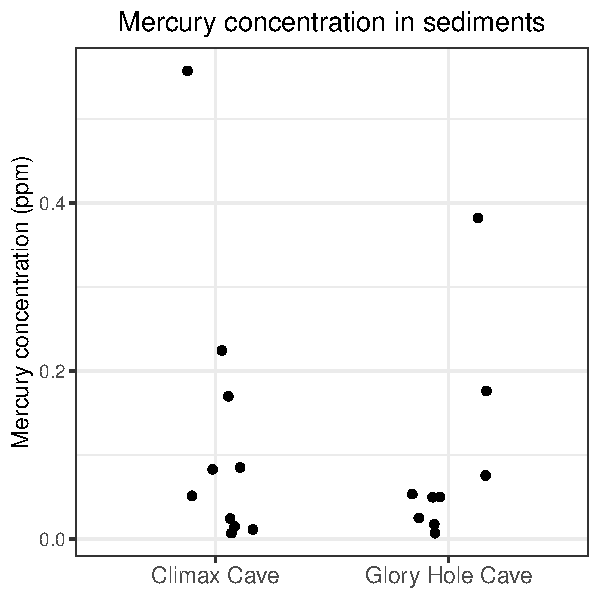
\includegraphics[height=4.0in]{dotplot_compare_sediment}
  \caption{Comparing the sediment concentrations}
  \label{fig:dotplot_compare_sediment}
\end{figure}

Because of the small sample sizes and the presence of outliers, we
cannot use the common statistical procedures, like the t-test.
Instead, we use a non-parametric test (Fisher-Pitman permutation test)
to do a hypothesis test of whether the means are significantly
different.  Not surprisingly, given the dotplot in Figure
\ref{fig:dotplot_compare_sediment}, the difference is not
significantly different (p $\approx$ 0.68).  Just to satisfy my
curiosity, I also did a non-parametric test of the variances, which
were also not signficantly different.


\vspace{0.2in}


\noindent \textbf{Is it possible that bats in Climax Cave aren't
  getting past the barrel room?}

I wondered if possibly the bats in Climax Cave aren't getting further
into the cave than the barrel room and its immediate surroundings.
Let's assume they aren't, and so bat guano wouldn't have been able to
impact map locations 14-17.  Then, we exclude map locations 14-17, and
only utilize the sediments from Climax Cave map locations 2, 3, 5, and
11-13.  Figure \ref{fig:dotplot_compare_sediment_reduced} contains a
dotplot illustrating the mercury concentration in the sediments in
this reduced dataset.  Again, there is no significant difference in
mercury concentrations between the sediments in the first portion of
Climax Cave and the sediments in Glory Hole Cave (p $\approx$ 0.26).
\begin{figure}[hb]
  \centering
  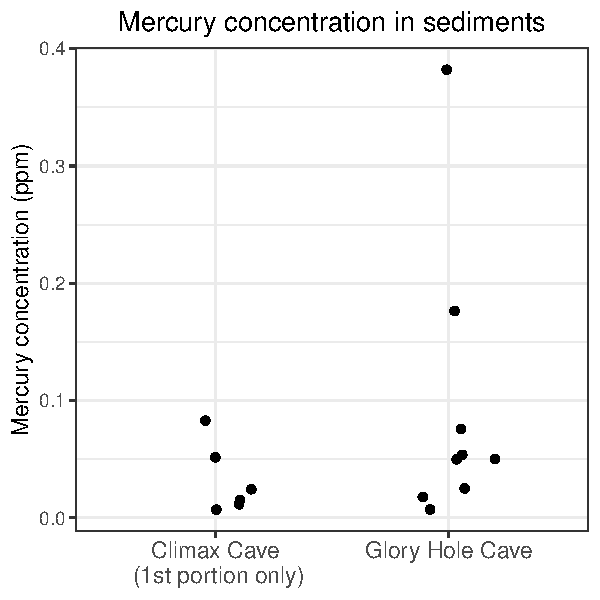
\includegraphics{dotplot_compare_sediment_reducedClimaxCave}
  \caption{Comparing the sediment concentrations between the first portion of Climax Cave and the entirety of Glory Hole Cave}
  \label{fig:dotplot_compare_sediment_reduced}
\end{figure}


\vspace{0.2in}


\noindent \textbf{Are mercury concentrations significantly different
  between sediment and guano in Climax Cave?}

Climax Cave has both guano and sediment samples, so we can compare
whether the average mercury levels in these two types of samples are
significantly different.  Figure \ref{fig:dotplot_climaxcave_by_area}
shows the mercury concentrations in both guano and sediment samples,
plotted by the cave area from which they originated.  The Tee Pee Room
is the only area of the cave from which we have a mix of the two types
of samples, with one sample from guano and one from sediment.  The
Barrel Room has only samples from guano.  Other than the one sample
from the Tee Pee Room, the sediment samples come from a variety of
other portions of the cave, and are the only samples from these other
areas.
\begin{figure}[hb]
  \centering
  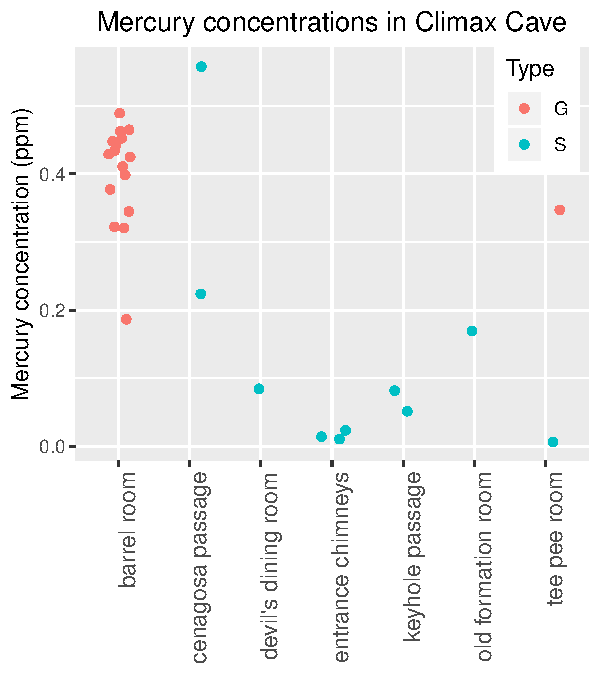
\includegraphics{dotplot_climaxcave_by_area}
  \caption{Concentrations of mercury in guano (G) and sediment (S) by area within Climax Cave}
  \label{fig:dotplot_climaxcave_by_area}
\end{figure}

This is a situation where the effect of sample type (guano
vs.\ sediment), if any, is \textit{confounded} with the effect of area
within the cave.  Looking at Figure
\ref{fig:dotplot_climaxcave_by_area}, one might suspect that the
mercury concentrations differ by location, and not necessarily by
sample type (guano vs.\ sediment).  Because we have a relatively small
number of samples in any one room outside of the Barrel Room, we can't
use statistical techniques to begin addressing the issue of whether
the mean concentrations are different among these seven areas of
Climax Cave.  On visual inpsection, it zdoes seem possible that there
are differences by location, as in the case of the 3 observations from
the Entrance Chimneys, which are quite similar to one another.

Statistically, when I compare mercury concentrations in guano with
mercury concentrations in sediment, I'm also comparing the Barrel Room
against all the other areas of Climax Cave (excepting the one guano
observation in the Tee Pee Room). 



\end{document}
